% CHIMERA-agent (MICCAI 2026) -- 6-page method description.
% Build: ./fetch-template.sh && make
%
% TODO before submission:
%   - affiliation, e-mail and team name (marked \todo{} below)
%   - the test-set row in Table 2, once the Sep 10 submission resolves
%   - verify volume/page fields in refs.bib
\documentclass[runningheads]{llncs}

\usepackage[T1]{fontenc}
\usepackage{graphicx}
\usepackage{booktabs}
\usepackage{amsmath}
\usepackage{xcolor}
\usepackage{tikz}
\usetikzlibrary{arrows.meta,positioning}
\usepackage[hidelinks]{hyperref}

\newcommand{\todo}[1]{\textcolor{red}{[#1]}}
\newcommand{\code}[1]{\texttt{\small #1}}

\begin{document}

\title{Most of a Scored Reasoning Trace Is a Supervised Target}
\subtitle{A deterministic entry to the CHIMERA-agent challenge}

\author{Austin M. Yunker}
\institute{Loyola University Chicago, Chicago IL, USA \\ \email{\todo{e-mail}}}

\maketitle

\begin{abstract}
The CHIMERA-agent challenge scores not only a clinical decision but the reasoning
trace accompanying it: a confidence level, a per-variable importance weighting, a
declared evidence-retrieval sequence, and a free-text rationale judged by a large
language model. We observe that $0.75$ of the per-case score on Tasks~1 and~2 is
computed by exact ordinal and set comparison against a urologist's annotation form,
and is therefore a \emph{supervised target} rather than a generation problem. We
build accordingly: the decision and every deterministically-scored field come from
a guideline stratification whose entire learned object is nine categorical labels,
and the rationale is templated against the judge's actual evidence context. No
language model runs at inference; the runtime dependencies are NumPy,
scikit-learn and Pydantic. The system reaches an overall validation ranking score
of $0.8061$ (Task~1 $0.7800$, Task~2 $0.8427$, Task~3 $0.7851$). We further report
a property of the challenge metric --- \code{cost\_aware\_tool\_score} is a
precision that returns $1.0$ for an empty declaration, making \emph{retrieving
nothing} weakly dominant --- which we document rather than exploit, and a set of
cross-validated negative results delimiting how much of the reasoning trace is
learnable at all.

\keywords{Prostate cancer \and Clinical decision support \and Agent evaluation
\and Reasoning traces \and Model Context Protocol}
\end{abstract}

\section{Introduction}

CHIMERA-agent~\cite{chimera} poses three prostate-cancer decision problems over
multimodal records from Radboudumc and Karolinska: whether to biopsy on MRI alone
(Task~1), how to treat given MRI and biopsy (Task~2), and time to biochemical
recurrence after prostatectomy (Task~3). Its distinguishing feature is that the
\emph{reasoning trace} is scored. Each Task~1/2 submission carries a confidence
level, a weighting of each clinical variable as
\code{not\_used}/\code{noted}/\code{important}/\code{decisive}, a declared sequence
of record sections retrieved through the Model Context Protocol
(MCP)~\cite{mcp}, and a free-text rationale graded by a G-Eval-style
judge~\cite{geval}.

The obvious reading is that this calls for a language agent: one model emits the
decision and narrates its own reasoning. Reading the released evaluator changes
that reading. The per-case score is a weighted sum of six components, and only one
of them --- the rationale, at weight $0.20$ --- is generated text. Confidence
($0.20$), variable weighting ($0.25$), important/decisive factor F1 ($0.15$), tool
efficiency ($0.15$) and section grounding ($0.05$) are all computed by exact
comparison against a urologist's annotation form. Those are supervised targets with
learnable structure. An agent asked to produce them by generation leaves measurable
points on the table, and --- more importantly for a clinical setting --- produces
an artefact whose correctness cannot be checked without running the judge.

We therefore describe a deliberately small, fully deterministic system that
separates \emph{deciding} from \emph{narrating} (Sect.~\ref{sec:method}) and report
its validation results (Sect.~\ref{sec:results}); a dominance property of the
challenge's own tool-efficiency metric, with the design rule we adopted so as not
to exploit it (Sect.~\ref{sec:metric}); and cross-validated negative results
bounding how much of the reasoning trace is predictable at all
(Sect.~\ref{sec:negative}) --- which we believe is the more useful contribution to
anyone designing the next such benchmark.

\section{Method}
\label{sec:method}

\subsection{Deciding, Acquiring, Narrating}

\begin{figure}[t]
\centering
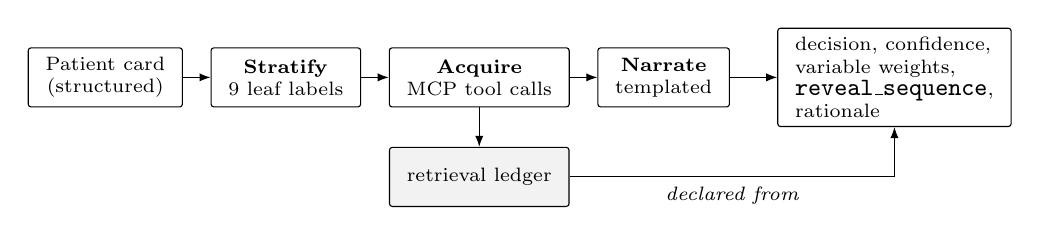
\begin{tikzpicture}[
  node distance=3.5mm,
  font=\scriptsize,
  box/.style={draw, rounded corners=1pt, align=center, minimum height=7.5mm,
              inner xsep=2.2mm},
  lbl/.style={font=\scriptsize\itshape},
  ar/.style={-{Latex[length=1.4mm]}}]

\node[box] (card) {Patient card\\(structured)};
\node[box, right=of card] (strat) {\textbf{Stratify}\\9 leaf labels};
\node[box, right=of strat] (acq) {\textbf{Acquire}\\MCP tool calls};
\node[box, right=of acq] (nar) {\textbf{Narrate}\\templated};

\node[box, below=5mm of acq, fill=black!5] (ledger) {retrieval ledger};

\node[box, right=6mm of nar, align=left] (out)
  {decision, confidence,\\variable weights,\\\code{reveal\_sequence},\\rationale};

\draw[ar] (card) -- (strat);
\draw[ar] (strat) -- (acq);
\draw[ar] (acq) -- (nar);
\draw[ar] (nar) -- (out);
\draw[ar] (acq) -- (ledger);
\draw[ar] (ledger) -| node[lbl, pos=0.25, below] {declared from} (out);
\end{tikzpicture}
\caption{The three stages. \code{reveal\_sequence} is emitted \emph{from} the
ledger of sections a tool call actually returned, so a section cannot be declared
unless it was retrieved. No language model runs at inference.}
\label{fig:arch}
\end{figure}

The system has three separable parts (Fig.~\ref{fig:arch}). A \emph{stratifier}
maps the case to a guideline leaf and looks up that leaf's decision. An
\emph{acquirer} retrieves the record sections the decision requires, over MCP, and
records what it retrieved. A \emph{narrator} writes the rationale from the
retrieved evidence. Nothing is learned end-to-end and no component is a language
model.

\paragraph{Stratification.}
Task~1 is stratified on PI-RADS~\cite{pirads} alone, into
\{\code{high} ($\geq 4$), \code{low}, \code{unknown}\}. Task~2 uses an EAU risk
stratification~\cite{eau} over biopsy status, ISUP grade, PSA and clinical stage,
into six leaves. Each leaf carries one fitted label. \emph{The entire learned
object is nine categorical values} --- three for Task~1, six for Task~2 --- chosen
to maximise the official metric under cross-validation. There is no per-case
learned function, which means every prediction the system makes can be explained by
naming its leaf, and a clinician can audit the model by reading a nine-row table.

Labels are fitted to the ranking metric rather than to accuracy, because the two
disagree: Task~1 ranks on $(\text{mean case score} + F_1^{\text{yes}})/2$, so a leaf
label trades decision accuracy against the reasoning components gated behind it.

\paragraph{Acquisition and reveal honesty.}
\code{reveal\_sequence} is self-reported, and the evaluator never inspects real MCP
traffic --- a declared retrieval is scored whether or not it happened. We treat
this as a constraint rather than an opportunity. Our MCP client exposes each case
as a store whose every successful section read is appended to a ledger, and the
declaration is emitted \emph{from} that ledger. A section can therefore be declared
only if a tool call returned it. Reveal honesty is structural rather than a
convention maintained by hand, and the optimisation problem we solve is which
evidence to \emph{acquire} --- a legitimate agent-design question --- rather than
what to claim afterwards.

The MCP client and server are hand-rolled over the standard library. The official
SDK's dependency tree (Pydantic, anyio, httpx, Starlette, uvicorn) does not fit the
offline submission image; conformance against the reference client is asserted in
the test suite instead, so that ``we speak MCP'' remains a protocol claim rather
than a stylistic one.

\paragraph{Narration.}
Two properties of the judge determine the rationale's wording, and neither is
guessable from the output schema. First, the judge's evidence context is the
narrative record sections, \emph{not} the structured patient card. A value that is
perfectly real --- sitting on the card we were handed --- reads to the judge as an
invented fact unless a report happens to state it too. Measured across the 348
released Task~1/2 cases, PI-RADS co-occurs in the reports 95--97\% of the time and
ISUP 100\%, but prostate volume only 48--58\%. The templates quote the former
freely and the latter never. Second, procedural meta-data (``Guideline basis:
\ldots'') is read by the judge as bookkeeping rather than reasoning, so the
guideline stratum opens the rationale as a clinical characterisation instead.

\subsection{Task 3: Ordering, Not Regression}

Task~3 ranks on Harrell's C-index~\cite{harrell} alone, so only the \emph{ordering}
of predicted recurrence times matters and the reasoning trace earns nothing. We
score each case with CAPRA-S~\cite{capras} and map it monotonically to months;
because the map is monotone, its constants cannot affect the result.

CAPRA-S is an integer score taking 12 distinct values over 75 training cases, which
guarantees ties, and the C-index banks a flat $0.5$ on every tied pair --- 104 of
1130 comparable pairs. We add the MRI-derived probability of clinically significant
cancer as a bounded tie-break,
\begin{equation}
\text{risk} = \text{CAPRA-S} + w \cdot p_{\text{csPCa}}, \qquad w = 0.99 ,
\end{equation}
where $w<1$ is a deliberate \emph{bound}, not a tuned weight: the term can reorder
cases within a CAPRA band and never across one. This makes the addition
calibration-free. It requires $p_{\text{csPCa}}$ only to beat a coin flip within a
band, not to be on Radboudumc's scale, and if a site's pipeline emits no such value
the term vanishes and behaviour is byte-identical to plain CAPRA-S. On training it
resolves the tied pairs at $0.663$ and lifts the C-index from $0.7372$ to $0.7522$.

\section{Results}
\label{sec:results}

\begin{table}[t]
\caption{Validation-phase results. Submission~1 is the guideline stratification;
Submission~2 splits one Task~2 leaf. Tasks~1 and~3 returned bit-identical scores
across the two submissions, confirming that the change was isolated and that the
platform is deterministic.}
\label{tab:val}
\centering
\begin{tabular}{lccc}
\toprule
 & Submission 1 & Submission 2 & $\Delta$ \\
\midrule
Task 1 ranking score      & 0.7800 & 0.7800 & $\pm$0.0000 \\
\quad case score / $F_1^{\text{yes}}$ & 0.7099 / 0.850 & 0.7099 / 0.850 & \\
Task 2 ranking score      & 0.6666 & \textbf{0.8427} & $+$0.1761 \\
\quad case score / weighted $F_1$ & 0.5966 / 0.737 & 0.7422 / 0.943 & \\
Task 3 ranking score (C-index) & 0.7851 & 0.7851 & $\pm$0.0000 \\
\midrule
\textbf{Overall} $(0.4/0.4/0.2)$ & 0.7356 & \textbf{0.8061} & $+$0.0705 \\
\midrule
Test set & \multicolumn{3}{c}{\todo{pending, Sep 10}} \\
\bottomrule
\end{tabular}
\end{table}

Table~\ref{tab:val} gives the validation trajectory. The single change between
submissions was a split of the Task~2 \code{positive\_intermediate} leaf on
ISUP grade~1, relabelling that branch from active treatment to active surveillance.

We report this change because of \emph{how} it was validated rather than its size.
Before submitting, we pre-registered an expected interval of $+0.046$ to $+0.057$
overall, derived from a leaf-purity estimate on training and a per-case price
computed from the metric's component weights. The realised gain was $+0.0705$,
above the band. Inspecting which cases moved shows why the mechanism was right and
the magnitude was not: exactly six cases changed, all six had previously been
wrong, all six moved to the ground-truth label, and there was no collateral damage.
The per-case price was predicted to within 6\%; only the leaf's prevalence was
underestimated, because it is three times commoner in the validation cohort (6/36)
than in training (4/72). A test cohort resembling training would therefore yield
roughly $+0.024$, not $+0.0705$ --- and we regard the honest projection, not the
leaderboard delta, as the result.

The system is small. The submission image installs three runtime dependencies with
\code{--no-deps}, carries no model weights and no language model, and the source is
40 Python modules under 1\,MB, covered by 177 test functions including MCP protocol
conformance, scorer parity against the official evaluator to $10^{-9}$, and an
offline test asserting no outbound connection under \code{--network none}.

\section{What the Metric Rewards}
\label{sec:metric}

\code{cost\_aware\_tool\_score} (weight $0.15$) is a precision,
$|A \cap R| / |A|$ for declared set $A$ and reference set $R$, and it returns
$1.0$ when $A = \emptyset$, on the reasoning that no unnecessary cost was incurred.
Under-retrieval is never penalised. The empty declaration is therefore
\emph{weakly dominant} on this component: it scores the maximum against any
reference, and a perfectly chosen retrieval set can only equal it, never beat it.
An agent that reads nothing is scored at least as well as one that retrieves
exactly what the urologist did.

\code{section\_grounding\_score} is the intended counterweight, but it carries only
weight $0.05$ and is bounded: variables readable from the patient card (PSA, age)
are grounded for free, and those whose sections lie outside the reveal vocabulary
(comorbidity, family history) are excluded as ungradable. An agent weighting only
those is fully grounded having read nothing, and collects both components at
maximum.

This is visible in our own scores, and the structure is a property of the metric
rather than of our system. Our tool score is $1.000$ on both tasks while Task~2
section grounding is $0.223$; on all 72 training Task~2 cases the reference
\code{reveal\_sequence} is itself empty, so the $0.223$ is a floor rather than
headroom, and raising it would trade a weight-$0.15$ component for a weight-$0.05$
one. We report the property rather than optimise into it --- the retrieval policy
is chosen first and the declaration generated from the ledger of what came back
(Sect.~\ref{sec:method}). A benchmark for evidence-seeking agents probably wants
recall in this term, or a floor on the reference set.

\section{Negative Results}
\label{sec:negative}

The deterministic components look like an attractive target: variable weighting and
factor F1 together carry weight $0.40$, they are scored without a judge, and they
cannot regress a decision. Our shipped weighting is nearly constant --- a handful of
patterns keyed on the predicted decision --- so per-case conditioning appears to
have obvious headroom. Conditioning each variable's weight on the single best case
feature raises modal agreement by $+0.030$ (Task~1) and $+0.093$ (Task~2)
\emph{in sample}, with the ISUP weight rising from $0.389$ to $0.694$.

None of it survives cross-validation (Table~\ref{tab:cv}). Task~1's best refinement
is worth $+0.0003$ overall; every Task~2 refinement is negative, because
conditioning on ISUP splits 72 cases across roughly 18 cells and the per-cell
estimate is noisier than the signal it recovers.

\begin{table}[t]
\caption{Six-fold cross-validated reasoning-component scores. Cells with fewer than
five rows fall back to the pooled modal vector. In-sample gains do not transfer.}
\label{tab:cv}
\centering
\begin{tabular}{lcccc}
\toprule
& \multicolumn{2}{c}{Task 1 ($n{=}91$)} & \multicolumn{2}{c}{Task 2 ($n{=}72$)} \\
\cmidrule(lr){2-3}\cmidrule(lr){4-5}
Weighting keyed on & var.\ weight & factor $F_1$ & var.\ weight & factor $F_1$ \\
\midrule
shipped blocks (in-sample)  & 0.8616 & 0.7526 & 0.8410 & 0.6881 \\
decision (shipped, CV)      & 0.8645 & 0.7330 & 0.8229 & 0.6512 \\
decision $\times$ PI-RADS   & 0.8685 & 0.7369 & --- & --- \\
decision $\times$ ISUP      & --- & --- & 0.8111 & 0.6315 \\
ISUP alone                  & --- & --- & 0.8184 & 0.6567 \\
\bottomrule
\end{tabular}
\end{table}

Three further negatives are worth recording. \emph{Missingness is not the rule
behind \code{not\_used}}: every variable is uniformly present or uniformly absent
across the cohort, so there is no within-variable split to exploit --- the
csPCa probability is marked \code{not\_used} on 67\% of Task~1 cases while always
being available. The annotation reflects clinical judgement, not availability.
\emph{Confidence is already at its ceiling}: it carries the largest component
weight ($0.20$) and is equally deterministic, and our constant emission scores a
cohort-level $\kappa$ of exactly zero --- yet constant \code{clear} \emph{is} the
cross-validated optimum on Task~1, because the minority classes are unrecoverable
from the features. \emph{Our own fitted blocks are mildly optimistic}: Task~2
in-sample $0.8410$ against $0.8229$ under cross-validation, which is approximately
the gap the validation cohort showed.

Aggregating, every remaining reasoning-component lever prices under $+0.002$
overall --- smaller than cross-validation seed variance. The one large lever left is
Task~1's six gate-failing cases, worth $+0.049$ overall, and it is the one we
judged unsafe: all six errors are false negatives, and PI-RADS $\geq 4$ is 69\%
positive in training but 100\% positive in validation, so fitting on training
suppresses exactly the calls the validation cohort rewards.

\section{Limitations and Conclusion}

The system is deliberately underpowered as a clinical model: nine labels cannot
capture case-level nuance, and its Task~1 errors are concentrated in prior-positive
biopsy patients at high PI-RADS, a subgroup that splits near 50/50 and that no
feature we tested separates. Roughly 40\% of the test cohort comes from a second
institution, and our strongest guard against that shift is that a nine-row lookup
table has little to overfit with; the bounded Task~3 tie-break was designed under
the same reasoning. Our reported gains come from a validation cohort whose leaf
prevalences differ markedly from training, and we have projected accordingly rather
than quoting the leaderboard delta.

The broader claim we would defend is methodological. When a benchmark scores a
reasoning trace, most of that trace may be an annotation form rather than an act of
reasoning, and treating it as a supervised target is both higher-scoring and more
auditable than generating it. The parts that genuinely require judgement are then
isolated and small enough to measure honestly --- which is how we came to report
that most of them are not learnable from these data at all.

\medskip
\noindent\textbf{Code.} \url{https://github.com/AustinYunker/ChimeraAgent}
(Apache~2.0).

\noindent\textbf{Data and embargo.} Results here use the CHIMERA-agent public
training and validation data under CC~BY-NC-SA~4.0 and are reported under the
challenge's publication embargo; the challenge publication is cited as required.

\begin{thebibliography}{8}

\bibitem{chimera}
CHIMERA-agent challenge, MICCAI 2026.
\url{https://chimera-agent.grand-challenge.org/}

\bibitem{mcp}
Anthropic: Model Context Protocol specification (2024).
\url{https://modelcontextprotocol.io}

\bibitem{geval}
Liu, Y., Iter, D., Xu, Y., Wang, S., Xu, R., Zhu, C.: G-Eval: NLG evaluation using
GPT-4 with better human alignment. In: EMNLP (2023)

\bibitem{pirads}
Turkbey, B., et al.: Prostate Imaging Reporting and Data System version 2.1.
European Urology \textbf{76}(3), 340--351 (2019)

\bibitem{eau}
Mottet, N., et al.: EAU-EANM-ESTRO-ESUR-SIOG guidelines on prostate cancer.
European Urology \textbf{79}(2), 243--262 (2021)

\bibitem{capras}
Cooperberg, M.R., Hilton, J.F., Carroll, P.R.: The CAPRA-S score: a straightforward
tool for improved prediction of outcomes after radical prostatectomy.
Cancer \textbf{117}(22), 5039--5046 (2011)

\bibitem{harrell}
Harrell, F.E., Lee, K.L., Mark, D.B.: Multivariable prognostic models.
Statistics in Medicine \textbf{15}(4), 361--387 (1996)

\end{thebibliography}

\end{document}
